\documentclass[10pt,letterpaper]{article}
\usepackage[T1]{fontenc}
\usepackage{lmodern,microtype}
\usepackage[margin=1in,headheight=14pt,headsep=16pt,footskip=26pt]{geometry}
\usepackage{amsmath,amssymb,amsthm,graphicx,booktabs,tabularx,array}
\usepackage[font=small,labelfont=bf]{caption}
\usepackage{enumitem,titlesec,fancyhdr,xcolor}
\usepackage[round,authoryear]{natbib}
\usepackage[colorlinks=true,linkcolor=blue!50!black,citecolor=blue!50!black,urlcolor=blue!50!black,breaklinks=true]{hyperref}
\usepackage{url}
\urlstyle{same}
\hypersetup{pdftitle={Depth Robustness Across Architectures: An Audit of Layer Dropout},pdfauthor={Gradient Dissent - independent research note},pdfsubject={Analytical audit and local/A100 replication of layer-dropout depth robustness}}
\titleformat{\section}{\large\sffamily\bfseries}{\thesection}{1em}{}
\titleformat{\subsection}{\normalsize\sffamily\bfseries}{\thesubsection}{1em}{}
\titlespacing*{\section}{0pt}{15pt}{8pt}
\titlespacing*{\subsection}{0pt}{11pt}{6pt}
\setlength{\parindent}{0pt}\setlength{\parskip}{5pt}
\setlength{\textfloatsep}{12pt}\setlength{\floatsep}{10pt}
\setlength{\bibsep}{5pt}
\setlist{nosep,leftmargin=18pt}
\pagestyle{fancy}\fancyhf{}\fancyhead[C]{\small\sffamily Depth Robustness Across Architectures: An Audit of Layer Dropout}\fancyfoot[C]{\thepage}
\fancypagestyle{firstpage}{\fancyhf{}\fancyhead[L]{\small\sffamily\bfseries GRADIENT DISSENT}\fancyhead[R]{\small\sffamily Independent research note}\fancyfoot[C]{\thepage}}
\newtheorem{proposition}{Proposition}
\newcommand{\CE}{\operatorname{CE}}
\newcommand{\E}{\mathbb{E}}
\newcommand{\Var}{\operatorname{Var}}
\newcommand{\source}{\href{https://github.com/yaroslavvb/gradient-dissent}{Code, measurements and reproducible analysis}}
\newcommand{\ResultRows}{%
GPT & Dense & 3.512 & 7.711 & +4.199 & 38.48 & 15.38 \\
GPT & Constant ILD & 3.645 & 3.738 & +0.093 & 37.01 & 36.31 \\
GPT & Decreasing ILD & 3.736 & 3.852 & +0.116 & 36.06 & 35.22 \\
\addlinespace
ConvNeXt & Dense & 3.457 & 8.156 & +4.699 & 51.34 & 14.19 \\
ConvNeXt & Constant ILD & 2.745 & 2.648 & -0.096 & 54.62 & 51.01 \\
ConvNeXt & Decreasing ILD & 2.891 & 2.775 & -0.116 & 54.12 & 50.62 \\
\addlinespace
ViT & Dense & 3.079 & 2.244 & -0.836 & 47.04 & 46.68 \\
ViT & Constant ILD & 2.713 & 2.155 & -0.558 & 49.55 & 50.57 \\
ViT & Decreasing ILD & 2.561 & 2.209 & -0.353 & 48.40 & 48.77 \\%
}

\newcommand{\EffectRows}{%
GPT & Constant ILD & $-4.106$ & $[-5.390,\ -2.823]$ \\
GPT & Decreasing ILD & $-4.083$ & $[-5.364,\ -2.802]$ \\
ConvNeXt & Constant ILD & $-4.795$ & $[-10.705,\ +1.116]$ \\
ConvNeXt & Decreasing ILD & $-4.815$ & $[-10.913,\ +1.283]$ \\
ViT & Constant ILD & $+0.278$ & $[+0.226,\ +0.330]$ \\
ViT & Decreasing ILD & $+0.483$ & $[+0.389,\ +0.578]$ \\%
}

\begin{document}
\thispagestyle{firstpage}
\vspace*{0pt}
\begin{center}
{\LARGE\sffamily\bfseries Depth Robustness Across Architectures:\\[5pt] An Audit of Layer Dropout}\par
\vspace{10pt}
{\normalsize Gradient Dissent}\par
{\small Independent replication and analytical audit \quad 9 September 2026}\par
\vspace{5pt}
{\small\href{https://yaroslavvb.github.io/gradient-dissent/significance/}{Interactive overview}\quad$\vert$\quad\source}
\end{center}
\vspace{2pt}
\textbf{Abstract.}
Layer dropout can produce useful shallower subnetworks, but pruning robustness, absolute quality and computational efficiency are distinct claims. We audit \emph{Don't Drop Dropout} through analytical checks, two local toy studies and A100 experiments with a 124M-parameter GPT, an 85M-parameter vision transformer (ViT) and a 28M-parameter ConvNeXt. Each larger setting compares dense training with constant and decreasing depth-dependent dropout, using validation-only learning-rate selection and three paired final seeds. GPT shows lower pruning damage with worse full-model quality at our short budget. ConvNeXt shows large observed benefits with wide primary intervals. ViT exposes a metric reversal: dropout yields lower mean pruned cross-entropy, yet looks worse on loss change from full because dense training benefits more from prefix deletion. Intermediate deletion gives a different result at the same depth. Local smaller dense controls remain competitive. Separately, a scalar counterexample disproves an expectation-preservation argument under the printed shared-mask implementation. These findings support conditional usefulness while motivating joint reporting of full quality, pruned quality, mask structure and uncertainty. Training executes branches before masking; no training-compute, latency or energy saving is established.
\begin{figure}[!h]
\centering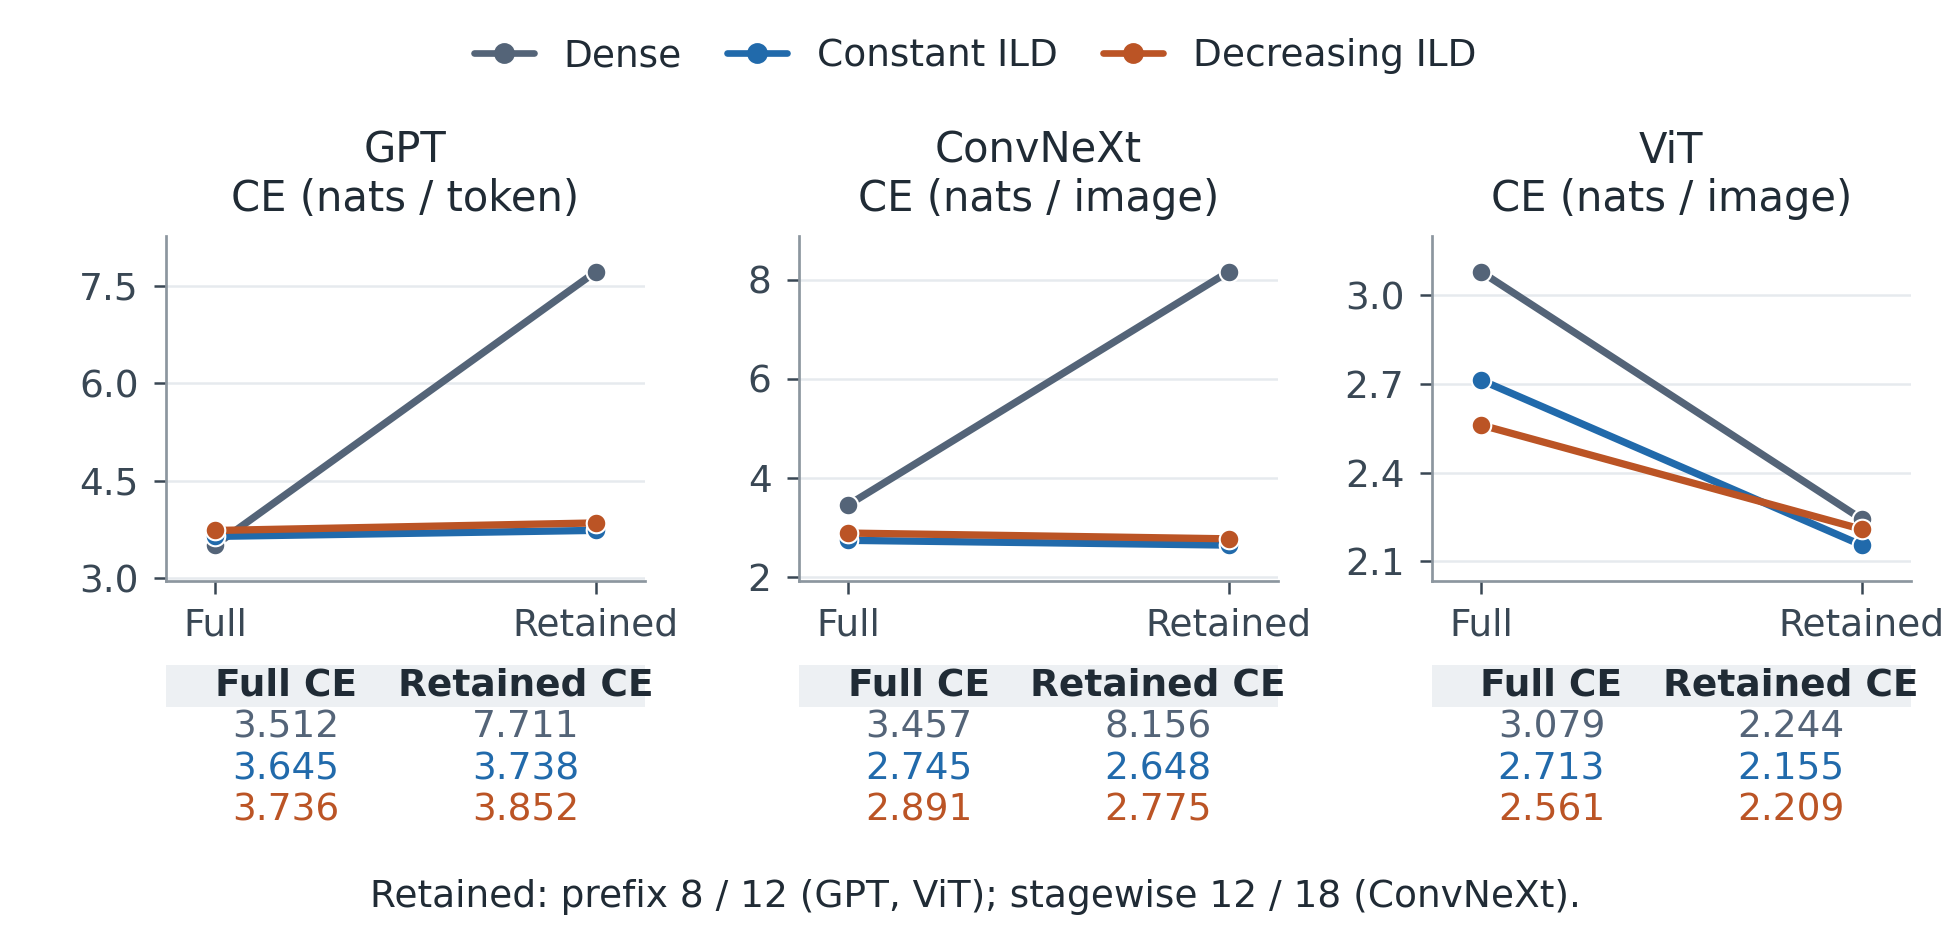
\includegraphics[width=\linewidth]{figures/fig1_full_to_pruned_ce.png}
\caption{\textbf{The starting point changes the interpretation.} Mean cross-entropy before and after the predefined two-thirds-depth intervention, across three training seeds. Lower is better. GPT and ConvNeXt dense models worsen substantially; dense ViT improves more than its dropout counterparts while retaining worse mean pruned CE. Lines connect measured endpoints, not a training trajectory. Axes differ across tasks; token and image CE magnitudes are not directly comparable. Paired uncertainty appears in Table~\ref{tab:effects}.}
\label{fig:overview}
\end{figure}

\clearpage
\section{Introduction}
Training a model that tolerates missing computation is attractive because the same checkpoint can serve several deployment budgets. The relevant claim is stronger than observing that a damaged model still produces outputs, but weaker than establishing that its truncated version is the best model for that budget. Three questions should be separated. First, how much does a fixed intervention change a checkpoint's performance? Second, how good is the resulting predictor in absolute terms? Third, was training and deploying this family preferable to alternatives, including a smaller model trained directly?

\citet{target} study layer dropout in modern causal language models, varying mask granularity, depth distribution, temporal schedules and scaling rules. The reviewed arXiv version is a slightly extended ICML 2026 paper. Its empirical value is that structured depth noise can improve selected training tradeoffs and leave useful subnetworks even when dropout is annealed away. This differs from treating dropout solely as a response to classic overfitting. The reported sweep includes more than 2,400 runs and models up to 8.2B parameters. These scale claims belong to the source paper, not to our experiments.

We evaluate selected mechanisms in a smaller, independently implemented setting. Our larger study spans a causal language transformer, a bidirectional image transformer and a convolutional network. It is an architectural transfer test, not a reproduction of the source paper's corpus, CompleteP parameterization, hardware or training duration. The local studies provide exhaustive subset evaluation and directly trained smaller controls that are absent from the A100 arm.

The principal empirical insight is a reversal in ViT. Relative loss change favors the dense baseline at a prefix exit, while mean absolute pruned loss and accuracy favor dropout. This is not a logical contradiction: subtracting each treatment's own full-model loss changes the question. A second finding is that intermediate deletion and suffix deletion behave very differently, even when eight of twelve blocks remain. A third contribution is an exact counterexample to a printed expectation-preservation rationale. Together these results support a more precise interpretation of depth robustness rather than a new dropout algorithm.

\section{Relationship to existing work}
Random residual-layer omission began in vision. \citet{huang} trained randomly shortened residual networks and evaluated the deep model. \citet{layerdrop} connected structured transformer dropout to extracting shallower subnetworks without fine-tuning. Thus neither transfer to CNNs nor inference with fewer transformer layers is a new general principle. The original ConvNeXt implementation already includes depth-increasing stochastic depth and LayerScale \citep{convnext}; our experiment examines an adapted training recipe and particular pruning interventions.

Temporal scheduling also has important precursors. Progressive Layer Dropping increases omission during transformer training \citep{progressive}. RaPTr grows random subnetworks toward the full model \citep{raptr}, closely anticipating the motivation for decreasing omission. Its preprint appeared in 2024 and its conference publication is ICLR 2025. The target paper adds a continuous depth/time recipe, per-sequence granularity, parameterization experiments and causal-LM inference analysis. The distinction is in the tested combination and evidence, not the invention of growing active capacity.

LayerSkip combines depth-increasing dropout with an explicit early-exit objective and self-speculative decoding \citep{layerskip}. The target paper investigates useful subnetworks without requiring that auxiliary objective during its main pretraining recipe. Our studies use a single existing output head and no auxiliary loss, adaptation or self-speculative decoder. They therefore do not reproduce LayerSkip's full procedure or establish decoding acceleration.

Finally, CompleteP studies depth/width parameterization and feature learning \citep{completep}, while Power Lines studies batch-size and weight-decay scaling \citep{powerlines}. These contextualize the target paper's optimizer-transfer rules. Our ordinary parameterization deliberately leaves that part of the source recipe untested. A negative transfer result here would not isolate a failure of CompleteP, and a positive result would not verify its theoretical assumptions.

\clearpage
\section{Analytical audit}
\subsection{Local unbiasedness does not establish shared-block unbiasedness}
For deterministic input $h$, a fixed residual branch $f$ and $M\sim\mathrm{Bernoulli}(\rho)$, inverted dropout satisfies
\begin{equation}
\E_M\!\left[h+\frac{M}{\rho}f(h)\mid h\right]=h+f(h).
\label{eq:local}
\end{equation}
The target paper's preferred block setting shares a mask between attention and feed-forward residual updates, while scaling each separately (printed Eq.~6 and \S6.1). The second branch's input then depends on the same mask multiplying its output. Equation~\ref{eq:local} cannot be applied twice while treating that input as independent of the mask.

\begin{proposition}
Consider a scalar two-sublayer residual block with fixed input $x$, attention $ax$, feed-forward map $bz$, and a shared mask $M\sim\mathrm{Bernoulli}(\rho)$, where $0<\rho\leq1$. If each training residual update is scaled by $M/\rho$ and evaluation uses scale one, then
\begin{equation}
\E[y_{\mathrm{train}}]-y_{\mathrm{eval}}=abx\frac{1-\rho}{\rho}.
\label{eq:gap}
\end{equation}
\end{proposition}
\begin{proof}
Writing $z=x+(M/\rho)ax$ gives
\begin{align}
y_{\mathrm{train}}&=z+(M/\rho)bz
=\left[1+(M/\rho)(a+b)+(M/\rho)^2ab\right]x,\\
\E[y_{\mathrm{train}}]&=\left[1+a+b+ab/\rho\right]x,
\end{align}
since $M^2=M$. Evaluation instead gives $[1+a+b+ab]x$. Subtraction yields Equation~\ref{eq:gap}.
\end{proof}
For $a=b=x=1$ and $\rho=1/2$, mask-off training outputs 1 and mask-on training outputs 9. Their mean is 5, whereas dense evaluation outputs 4. This exact enumeration is also implemented in the repository. The result corrects the stated rationale under the printed implementation; it does not show that the paper's observed training outcomes are false. An implementation that differs from the printed equations would require a separate analysis.

Independent attention and feed-forward masks recover equality in this linear example. Applying one inverted mask to the aggregate dense block residual also preserves its conditional mean. Neither construction implies global equality for an arbitrary nonlinear network: in general $\E[f(H)]\ne f(\E[H])$. Equality of expected logits would not establish equality of expected cross-entropy either.

\subsection{The robustness endpoint contains a moving reference}
Let $Q_r$ be full-model CE for recipe $r$, and $P_r(S)$ its CE after retaining subset $S$. Define signed pruning change $D_r(S)=P_r(S)-Q_r$. Our primary paired treatment effect is
\begin{equation}
\Delta_r(S)=D_r(S)-D_0(S)
=[P_r(S)-P_0(S)]-[Q_r-Q_0],
\label{eq:endpoint}
\end{equation}
where $0$ denotes dense training. Negative $\Delta_r$ means lower signed change; if both $D$ values are negative, it can mean a larger improvement rather than less damage. Equation~\ref{eq:endpoint} is a difference-in-differences identity, not a new estimator or a causal identification theorem.

For ViT with constant ILD, $P_r-P_0\approx-0.088$ and $Q_r-Q_0\approx-0.366$. Consequently $\Delta_r\approx+0.278$: the pruned dropout model has lower mean loss, but less improvement relative to its own stronger full model. A robustness score cannot replace reporting both endpoints. Conversely, a weaker full model can make a small pruning change look favorable even when its final predictor is poor.

\clearpage
\section{Experimental design}
\subsection{Recipes and shared controls}
Index the $L$ prunable residual blocks by $\ell=0,\ldots,L-1$ and steps by $t=0,\ldots,T-1$. The A100 study compares dense training, constant increasing layer dropout (ILD) and decreasing ILD:
\begin{equation}
p_{\ell,t}^{\mathrm{const}}=0.4\frac{\ell}{L-1},\qquad
p_{\ell,t}^{\mathrm{decr}}=0.8\frac{\ell}{L-1}\left(1-\frac{t}{T-1}\right).
\label{eq:schedules}
\end{equation}
Both have average mask probability 0.2 over blocks and steps. The first block is always retained. Decreasing ILD ends with a dense step; there is no prolonged dense continuation. Equal average omission does not isolate temporal order because the maximum rates and distribution of noise also differ.

Masks are sampled per sequence or image. Transformers share a mask across their two residual updates, each using inverse-survival scaling; ConvNeXt has one branch per prunable block. Training computes every branch before applying the mask. Within each family, recipes receive identical training steps, batch sizes, data exposure and learning-rate search sizes. This is not a matched sparse-FLOP experiment. Masks and augmentation use independent generators so they do not consume the paired data stream's randomness. Evaluation bypasses omitted blocks in their original order, retains final normalization/head at scale one and performs no adaptation.

\begin{table}[h]
\centering\small
\caption{\textbf{A100 configurations.} Training presentations include repeat sampling. Image passes are equivalent presentations divided by 45,000, not shuffled epochs. Both image models use the same CIFAR-100 split.}
\label{tab:models}
\begin{tabularx}{\linewidth}{@{}lXXX@{}}\toprule
 & GPT & ViT & ConvNeXt\\\midrule
Parameters & 124,439,808 & 85,219,684 & 27,897,028\\
Blocks & 12 & 12 & 3,3,9,3 across stages\\
Width & 768 & 768 & 96,192,384,768\\
Input & 1,024 GPT-2 tokens & $32\!\times\!32$, $4\!\times\!4$ patches & $32\to64$ image resize\\
Data & WikiText-103 & CIFAR-100 & CIFAR-100\\
Steps / batch & 3,200 / 32 & 10,240 / 256 & 10,000 / 512\\
Presentations & 104,857,600 tokens & 2,621,440 images & 5,120,000 images\\
Primary retention & First 8 of 12 & First 8 of 12 & Stage prefixes 2,2,6,2\\\bottomrule
\end{tabularx}
\end{table}

The GPT implementation follows a pinned nanoGPT reference \citep{nanogpt}, with causal attention, twelve heads and tied embeddings. It uses ordinary GPT initialization, not CompleteP. Data use official WikiText-103 splits \citep{wikitext}, GPT-2 tokenization and document-contained sampling. The test panel comprises 246 disjoint windows and 251,904 target tokens; short articles and tails are omitted. This is not canonical full-corpus WikiText perplexity. Each run sees only 0.843 token presentations per parameter, far below the source paper's common 20-TPP regime.

ViT adapts the image-transformer family \citep{vit} with 64 patch tokens and mean pooling, without a class token. ConvNeXt uses its Tiny stage pattern \citep{convnext}; the stem and stage transitions always remain. CIFAR-100 \citep{cifar} is split into 45,000 training, 5,000 validation and 10,000 official test images. Training uses crop/flip augmentation; ConvNeXt then bilinearly resizes to 64 pixels, which adds no source-image information. Equivalent training exposure is 58.25 passes for ViT and 113.78 for ConvNeXt.

\clearpage
\subsection{Selection, replication and uncertainty}
Each architecture/recipe pair receives three full-horizon learning rates on tuning seed 1000. Final full-depth validation CE selects the winner, without test or pruned metrics. The 27 tuning runs precede 27 final runs on seeds 2000--2002. Eight of nine winners lie at grid boundaries; no post-test extension is made. Grids and optimizer settings appear in Appendix~\ref{app:protocol}.

The primary intervention is fixed in advance: first eight blocks for GPT/ViT, or stage prefixes 2,2,6,2 for ConvNeXt. Nine fixed interventions per final checkpoint yield 243 raw mask evaluations. The other masks test more aggressive thinning, three random subsets retaining the first block, and deletion of only the first block. These are distinct interventions, not additional independent training replicates. All masks are published, and none is selected using final test performance.

Contrasts average per-seed differences with 95\% Student-$t$ intervals ($n=3$, $df=2$, critical value 4.30265). Six primary intervals are unadjusted for multiplicity. Accuracy and other masks are secondary, also unadjusted. Intervals describe seed variation conditional on selected settings and fixed data, omitting tuning, split and dataset uncertainty. Three-seed intervals are fragile, not population-wide guarantees.

GPT same-seed initial weights match exactly. Vision models require a qualification: worker-dependent truncated-normal initialization produced two numerical variants. Separate untrained reconstructions match every observed hash for each declared seed, preserve post-initialization RNG state, and differ by at most $7.45\times10^{-9}$ per parameter. These are post hoc verification adjustments, not changes to executed training. Tiny differences do not prove identical trajectories or negligible effects on final scores. Appendix~\ref{app:audit} records the audit and its limits.

\section{A100 results}
\begin{table}[h]
\centering\small\setlength{\tabcolsep}{5pt}
\caption{\textbf{Full and primary-pruned quality.} Means across three seeds. CE is nats per target; accuracy is percent. GPT accuracy is token accuracy, unlike image top-1 accuracy. $D=P-Q$ is signed change. The primary retention keeps two-thirds of prunable blocks, not necessarily two-thirds of all compute.}
\label{tab:quality}
\begin{tabular}{@{}llrrrrr@{}}\toprule
 & & \multicolumn{3}{c}{Cross-entropy $\downarrow$} & \multicolumn{2}{c}{Accuracy $\uparrow$}\\
\cmidrule(lr){3-5}\cmidrule(l){6-7}
Model & Recipe & Full $Q$ & Pruned $P$ & Change $D$ & Full & Pruned\\\midrule
\ResultRows
\bottomrule\end{tabular}
\end{table}

\subsection{GPT reproduces pruning resilience with a quality cost}
At the eight-block exit, dense GPT incurs 4.199 nats of CE increase, versus 0.093 for constant ILD and 0.116 for decreasing ILD. The corresponding paired effects are $-4.106$ and $-4.083$ nats, with both primary intervals below zero (Table~\ref{tab:effects}). The retained predictors are substantially better after ILD than after dense training.

This flexibility has a full-model cost. Relative to dense training, intact CE increases by 0.133 [0.076, 0.191] for constant ILD and 0.225 [0.192, 0.257] for decreasing ILD. Full token accuracy declines by 1.47 and 2.42 percentage points. These results replicate a depth-robustness mechanism, not a universal full-quality improvement, and do not settle the much longer training regime of the source paper.

\clearpage
\subsection{ConvNeXt exhibits large but uncertain primary effects}
Keeping twelve of eighteen ConvNeXt residual blocks reduces dense accuracy from 51.34\% to 14.19\%. Constant ILD retains 51.01\% from 54.62\%; decreasing ILD retains 50.62\% from 54.12\%. The primary relative-CE effects average $-4.795$ and $-4.815$ nats. All three seed differences favor ILD, but both intervals include zero because between-seed effect variation is large.

Secondary paired pruned-accuracy gains are 36.82 [13.55, 60.10] and 36.43 [9.60, 63.26] percentage points. This is a large observed benefit with uncertain magnitude, not proof of a precisely estimated universal CNN effect. CE and accuracy again differ: pruning either ILD model slightly improves mean CE while reducing accuracy by approximately 3.5 points. Learned LayerScale stage means reach roughly 0.04--0.16 from initialization at $10^{-6}$. Residual scales remaining near initialization cannot explain the result, although their magnitudes alone do not measure branch contribution.

\begin{table}[h]
\centering\small
\caption{\textbf{Primary paired effects.} $\Delta=(P-Q)_{\mathrm{ILD}}-(P-Q)_{\mathrm{dense}}$. Negative denotes lower signed CE change. Positive ViT effects indicate less improvement from prefix pruning, not necessarily worse absolute pruned prediction. Intervals are unadjusted 95\% Student-$t$, $n=3$, $df=2$.}
\label{tab:effects}
\begin{tabular}{@{}llrr@{}}\toprule
Model & Recipe & Mean $\Delta$ & 95\% interval\\\midrule
\EffectRows
\bottomrule\end{tabular}
\end{table}
\begin{figure}[h]
\centering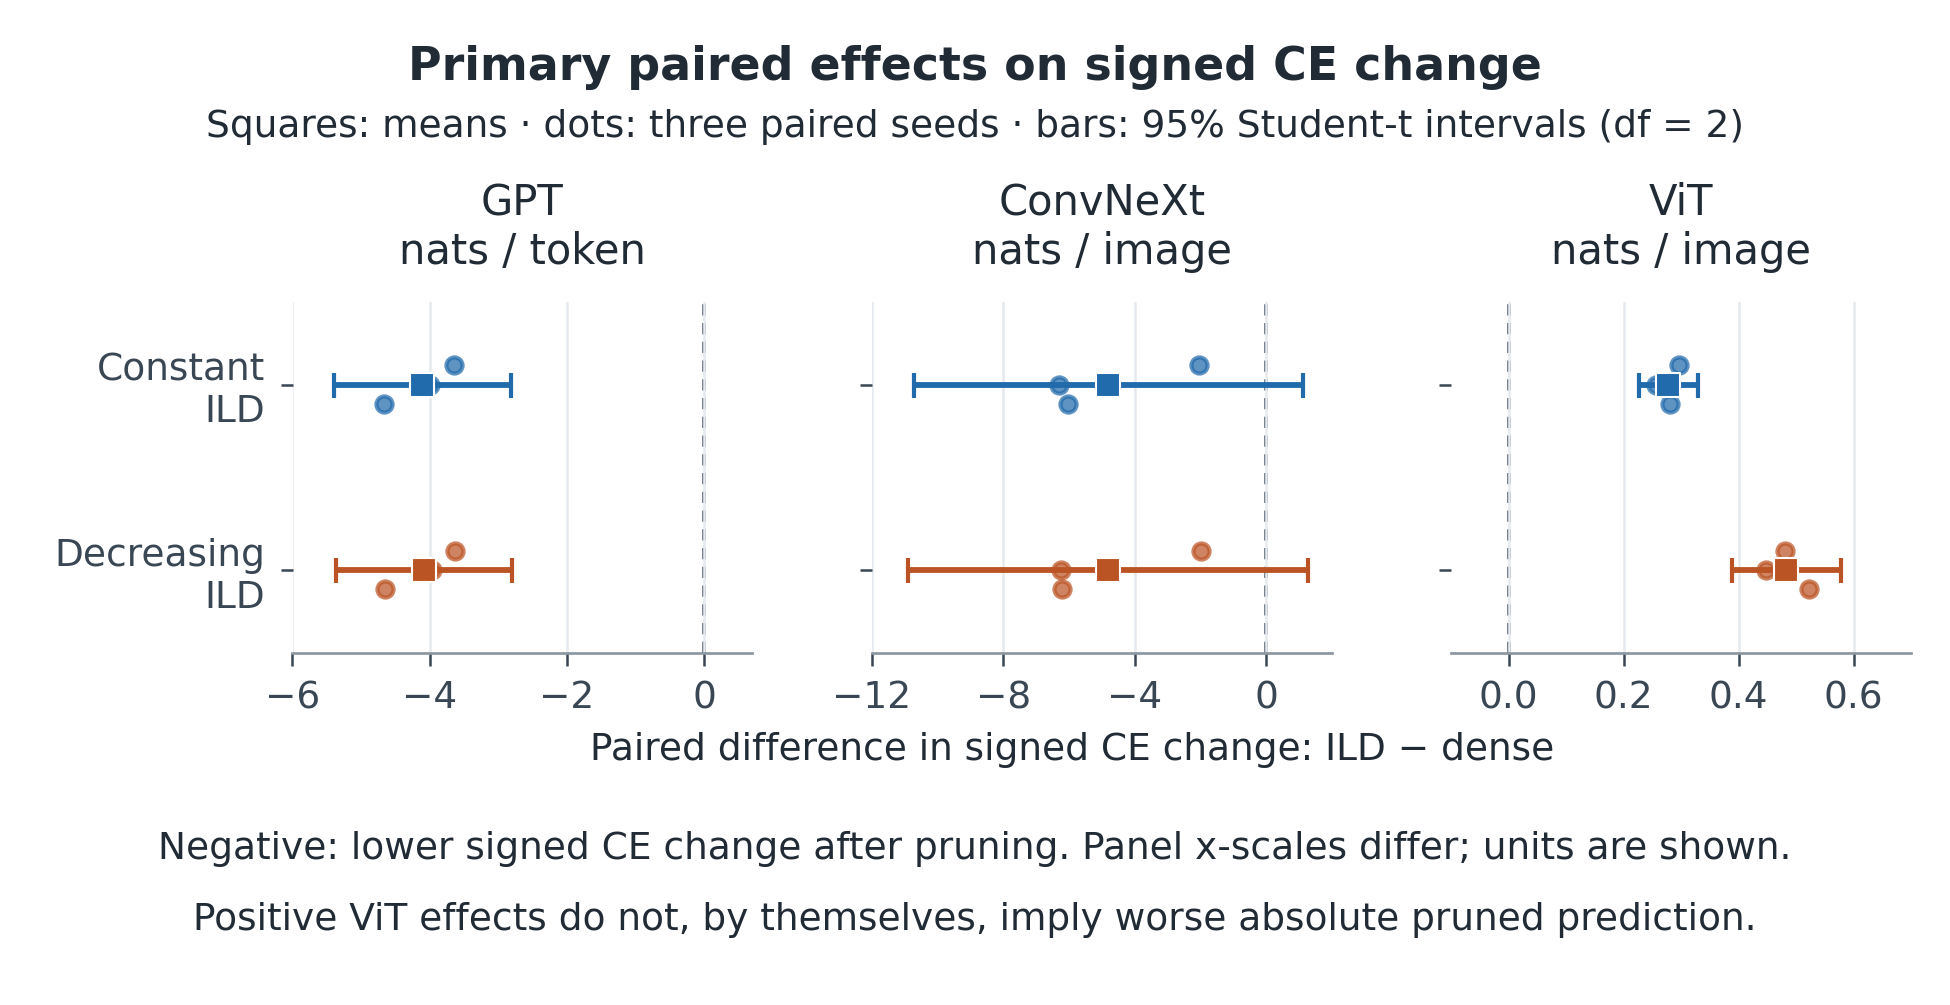
\includegraphics[width=\linewidth]{figures/fig3_primary_paired_effects.png}
\caption{\textbf{Observed effects and seed uncertainty.} Points show individual paired training-seed differences; intervals summarize their mean. Large ConvNeXt averages coexist with wide intervals. ViT reverses the sign at the predefined prefix intervention. Panel x-scales differ. The six intervals have no multiplicity adjustment.}
\label{fig:effects}
\end{figure}

\clearpage
\subsection{ViT separates predictor quality from relative change}
Dense ViT CE falls from 3.079 to 2.244 at the eight-block exit. Constant ILD falls from 2.713 to 2.155, and decreasing ILD from 2.561 to 2.209. Dense training therefore receives more improvement from prefix pruning, producing positive primary treatment effects of 0.278 [0.226, 0.330] and 0.483 [0.389, 0.578]. Nevertheless, both ILD recipes produce lower mean pruned CE. Their paired pruned-CE intervals include zero, so these small absolute-loss differences are not resolved by this experiment.

Pruned accuracy is 46.68\% for dense, 50.57\% for constant ILD and 48.77\% for decreasing ILD. Secondary paired gains are 3.89 [2.04, 5.75] and 2.09 [1.52, 2.67] points. Dense pruning's large CE improvement accompanies only a 0.36-point aggregate accuracy decline. Confidence or generalization problems are plausible explanations, but calibration error, logit magnitudes and per-example prediction agreement were not measured. Very low late minibatch losses alongside much higher held-out losses support a generalization concern; they do not identify its mechanism.

\begin{figure}[h]
\centering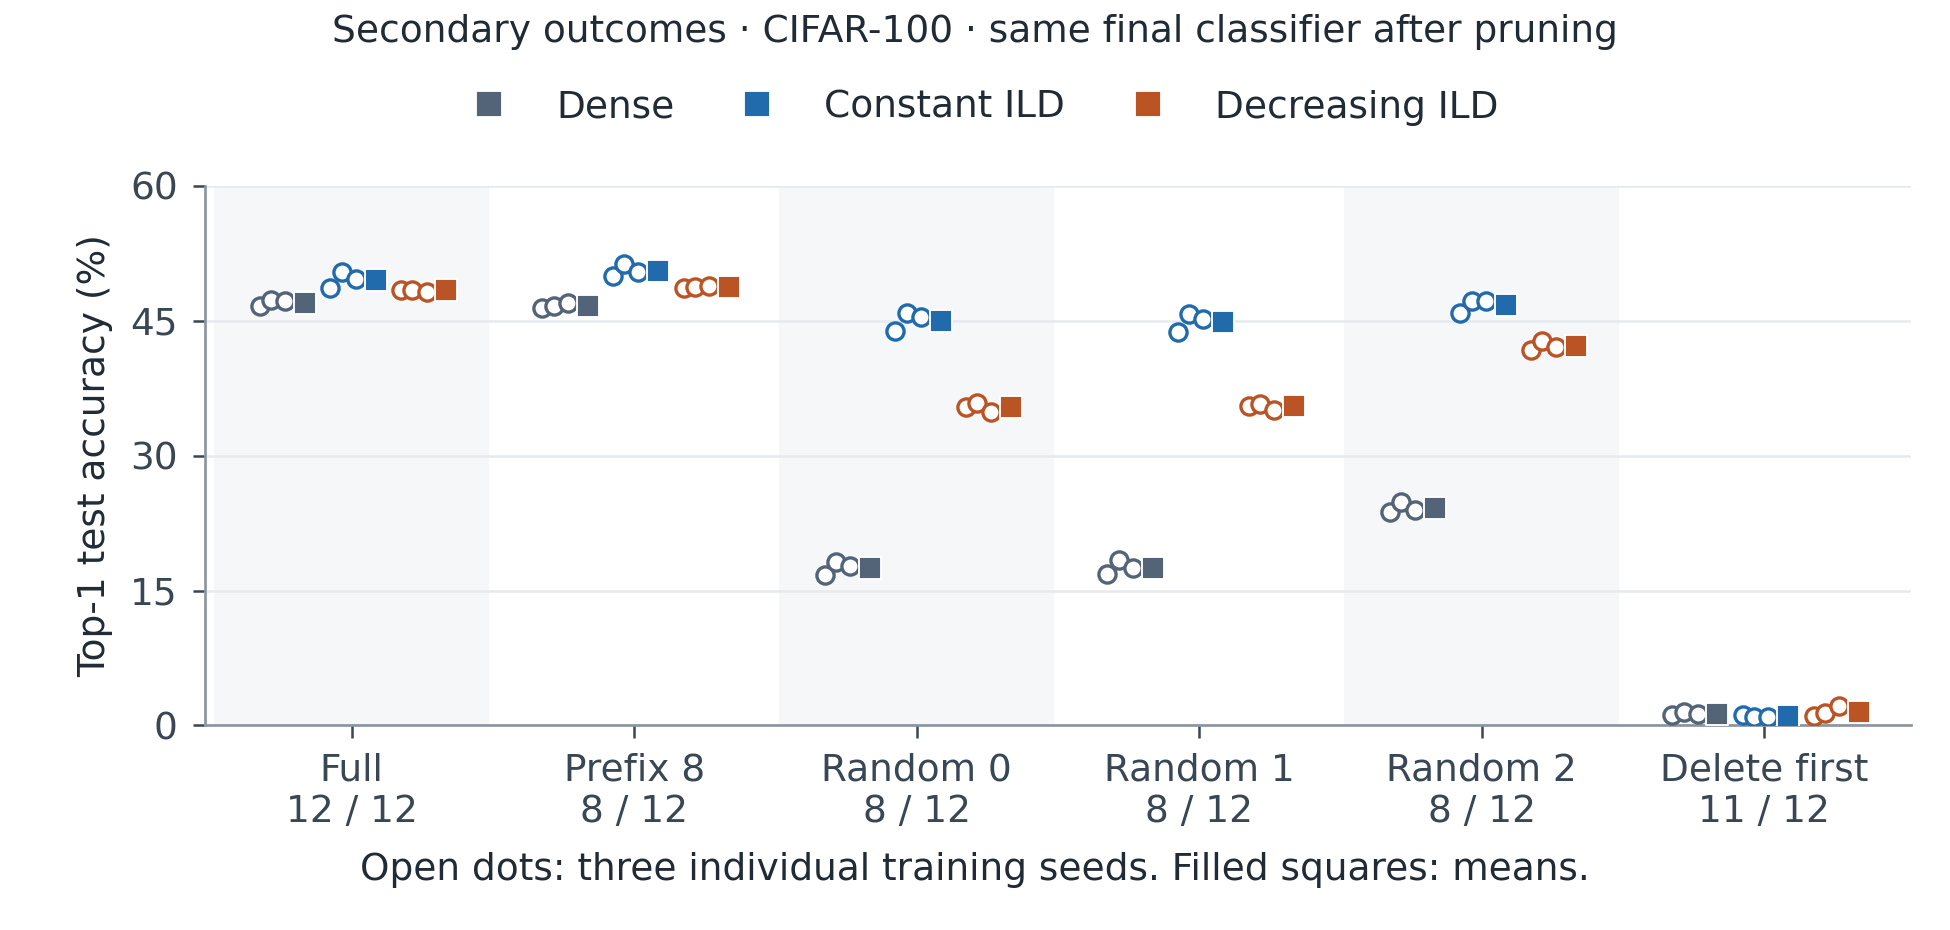
\includegraphics[width=\linewidth]{figures/fig2_vit_accuracy_secondary.png}
\caption{\textbf{Same depth, different deletion pattern.} ViT accuracy across fixed interventions. Random masks retain eight blocks at different original positions, always including the first; no layers are reordered. Markers show means and individual seed observations. These accuracy comparisons are secondary. Deleting the first block, which is never dropped in ILD training, is a separate boundary test and retains eleven blocks.}
\label{fig:masks}
\end{figure}

\subsection{Mask structure and schedule ranking limit transfer}
The three predefined random eight-block masks reduce dense ViT accuracy to 17.52--24.15\%, while constant ILD retains 44.90--46.75\% and decreasing ILD 35.37--42.23\%. All six secondary relative-CE intervals for these masks fall below zero. Thus the positive ViT primary effects do not generalize even to other masks at the same retained depth. Prefix exits and intermediate deletion probe different dependencies.

Deleting only the first block leaves ViT near 1\% image accuracy and GPT near 1--3\% token accuracy. ConvNeXt ILD accuracy falls to 24.93\%/17.85\%, versus dense 37.56\%. This intervention is outside the ILD training mask support. The recipe cannot be summarized as robustness to arbitrary missing blocks.

Nor is decreasing dropout uniformly better. Constant ILD has lower mean full and primary-pruned CE for GPT and ConvNeXt. Decreasing ILD has the best ViT full CE, whereas constant ILD has better prefix-eight CE and accuracy. At prefix four, ViT accuracy instead favors decreasing ILD, 47.65\% versus 45.75\%. These schedule comparisons are descriptive; equal mean mask probability is not a controlled isolation of a terminal dense phase.

\clearpage
\section{Local controls: useful subnetworks are not necessarily the best small models}
The local studies evaluate a six-block character transformer and a six-block residual MLP on scikit-learn's $8\times8$ digits. The language model has width 64, four heads and context 64, with 819,200 training targets per run from Tiny Shakespeare. Its fixed test panel has 128 windows and 8,192 targets. The digits split contains 1,078 training, 359 validation and 360 test examples, with 76,800 training presentations per run. This is neither MNIST nor a writer-disjoint split.

Each treatment searches five learning rates on two tuning seeds, then evaluates five separate final seeds. The retained design contains 90 tuning and 45 final runs, including an alternating-dropout arm in language. Six-block checkpoints undergo exact enumeration of all 63 nonempty layer subsets. The complete study has 2,315 subset evaluations; masks are aggregated within seed before uncertainty is calculated. No auxiliary heads, calibration or fine-tuning are used. These are local mechanism checks with matched data exposure, not matched computational cost.

\begin{table}[h]
\centering\small\setlength{\tabcolsep}{5pt}
\caption{\textbf{Local prefix-four results.} Mean CE across five seeds; paired effects use $df=4$ Student-$t$ intervals. Character CE and image CE have different units. Full-depth CE superiority over dense is unresolved locally.}
\label{tab:local}
\begin{tabular}{@{}llrrl@{}}\toprule
Task & Recipe & Full CE & Prefix-4 CE & Paired $\Delta$ [95\% interval]\\\midrule
Character LM & Dense6 & 2.11227 & 2.16210 & Reference\\
 & Constant ILD & 2.11229 & 2.11563 & $-0.04648\ [-0.06191,-0.03105]$\\
 & Decreasing ILD & 2.11887 & 2.12538 & $-0.04331\ [-0.05874,-0.02787]$\\
 & Alternating & 2.11032 & 2.13835 & $-0.02180\ [-0.04448,+0.00089]$\\\addlinespace
Digits & Dense6 & 0.07996 & 0.15629 & Reference\\
 & Constant ILD & 0.07837 & 0.08880 & $-0.06589\ [-0.08439,-0.04739]$\\
 & Decreasing ILD & 0.07996 & 0.08858 & $-0.06771\ [-0.08579,-0.04962]$\\\bottomrule
\end{tabular}
\end{table}

The local early-exit effects are favorable for both ILD schedules (Table~\ref{tab:local}). However, a separately trained smaller dense model has lower mean CE than either corresponding truncated ILD model (Table~\ref{tab:small}). The saved summaries do not contain direct paired smaller-versus-ILD superiority intervals; these are descriptive comparisons. The point is not that a small dense model always wins. It is that robustness to pruning a larger model does not establish the best way to obtain a particular deployment model.

\begin{table}[h]
\centering\small
\caption{\textbf{Direct smaller-model controls.} Descriptive mean CE, with lower being better. All models receive the same training exposure within each task. The A100 study contains no corresponding smaller dense controls.}
\label{tab:small}
\begin{tabular}{@{}lrrrl@{}}\toprule
Task / desired depth & Smaller dense & Constant ILD & Decreasing ILD & Parameters: small / six-block\\\midrule
Character LM / 4 & 2.10299 & 2.11563 & 2.12538 & 212,480 / 312,448\\
Digits / 3 & 0.08279 & 0.11875 & 0.10872 & 55,050 / 105,162\\\bottomrule
\end{tabular}
\end{table}

The smaller language model uses its own depth-specific initialization, including residual projection scale $0.02/\sqrt{2L}$; it does not share identical prefix weights with the six-block model. Digits constructs six blocks before slicing to three, preserving the initial prefix and head. The digits study also has a development qualification: an initial grid produced test results before a validation-triggered grid extension. The retained final design and archived earlier runs are disclosed; effect magnitudes changed. This local history should not be described as an untouched confirmatory protocol.

\clearpage
\section{From statistical flexibility to useful computation}
\subsection{What the original paper supports}
The source paper provides substantial evidence that its chosen layer-dropout recipe can leave useful pruned language models. Its full-model outcomes are more mixed. Table~5 reports validation CE of 1.849 dense versus 1.836 dropout at 1.8B parameters and 15\% nominal block-FLOP savings. At 3.9B, CE is 1.732 versus 1.745 with 20\% nominal savings: a quality/compute tradeoff. Its largest 8.2B row has no matched dense control. These observations neither negate the recipe nor support an unqualified improvement at every scale \citep[Table~5]{target}.

The distinction between block work and end-to-end efficiency matters. For the depth/time schedule in Equation~\ref{eq:schedules}, replacing the initial maximum 0.8 by $p_{\max}$ gives mean omission $p_{\max}/4$. The paper's $p_{\max}=0.99$ therefore corresponds to 24.75\% average omission of equal-cost nonembedding block work, conditional on actual skipping. It is not a measured 24.75\% reduction in total training time or energy. Unchanged output projections, optimizer traffic, communication and routing overhead remain.

A fixed cumulative-FLOP checkpoint comparison also differs from separately training a dense control to a fixed budget with its own terminal cooldown and tuned hyperparameters. Such controls, and a size sweep of smaller dense models, are needed to establish a compute frontier. Our A100 experiment does not provide them. Similarly, lossless self-speculation preserves the distribution of its own target model under an exact verifier; it does not restore the quality of a different dense-trained target.

\subsection{Connection to locality and energy objectives}
The \href{https://yaroslavvb.github.io/gyroscope/meetings/2026-09-07-061a993a3e32a40a.html}{public Sutro meeting notes of 7 September 2026} motivate charging data movement and occupied state, not only arithmetic. Layer dropout provides a concrete way to test the distinction between statistically useful sparsity and physically economical sparsity. If each of $B$ examples independently drops a layer with probability $p$, the probability that some example still needs that layer is
\begin{equation}
\Pr(\text{layer needed somewhere in batch})=1-p^B.
\end{equation}
At $p=1/2$ and $B=32$, this is $1-2^{-32}$, effectively one, despite half of example-layer computations being omitted in expectation. A batch-shared mask instead needs the layer with probability $1-p$. This is a probability identity, not an estimate of physical transfers: caches, weight placement and optimizer semantics determine actual traffic.

A useful follow-up would compare per-example, grouped and batch-wide masks at matched predictive quality, with genuinely bypassed execution. It should charge gathers, scatters, mask storage, gradients and optimizer state, while measuring time, energy and peak live memory separately. A schedule that becomes dense can reduce average active work without reducing the dense endpoint's peak memory. Static compaction of a chosen subnetwork and resident execution with bypasses also have different storage and movement costs.

For repeated deployment, the appropriate objective includes preparation and use: $E_{\mathrm{total}}(N)=E_{\mathrm{fit}}+E_{\mathrm{search/adapt}}+N E_{\mathrm{predict}}$. The meeting's proposed transductive digit task instead requires an explicit finite end-to-end boundary; an indefinite deployment amortization cannot be assumed. Neither our local digits study nor our A100 work measures that benchmark. The proposal is to add physical accounting to a statistically controlled comparison, not to equate a FLOP count or dollar bill with energy.

\clearpage
\section{Limitations and decisive follow-up experiments}
Our evidence is restricted to selected architectures, datasets, schedules and training budgets. Both larger vision models share CIFAR-100. GPT receives fewer than one token presentation per parameter, while the image models repeatedly sample a small dataset. Their late training-versus-held-out loss gaps make stronger augmentation, validation-selected regularization and longer or differently scheduled training important follow-ups. These limitations apply to our runs rather than establishing flaws in the source paper's experiments.

Three final seeds give unstable interval widths and do not characterize rare failures. Only one independent tuning seed is used at A100 scale, and eight of nine winners occur at a grid boundary. The quoted seed intervals omit model-selection uncertainty. Repeating the experiment with expanded validation-only searches and additional final seeds would test whether the observed architecture differences persist. The tiny vision initialization variants must remain disclosed even though they pass narrowly scoped numerical audits.

The primary masks are comparable as fractions of residual-block count, not as identical architectural operations. ConvNeXt preserves downsampling transitions and thins each stage; GPT/ViT discard a suffix. A fixed random mask panel samples only a small part of the subset space. The local exhaustive studies alleviate that limitation at toy scale but cannot establish the behavior of all A100 subsets.

The most informative next comparison is against directly trained target-depth models at both equal data exposure and equal measured compute. It would distinguish the convenience of choosing a subnetwork after training from efficiency at a known deployment depth. A second study should measure calibration and per-example prediction changes on validation data before testing an explanation for ViT's loss/accuracy divergence. A third should continue the annealed model through a substantial dense phase; the current final dense step is insufficient to test persistence after prolonged dense training. Finally, actual skipping kernels with matched masks are required before studying the energy/locality hypothesis.

\section{Conclusion}
Layer dropout produces useful subnetworks in these experiments, including non-causal image architectures. GPT's clear pruning benefit comes with a full-model quality cost; ConvNeXt's large observed gains have wide primary intervals; ViT demonstrates that the reference model and deletion pattern can reverse a robustness ranking. Local smaller dense controls show why a pruning result alone does not establish an optimal smaller predictor. The shared-mask counterexample narrows a mathematical justification without erasing the empirical findings.

The appropriate evaluation unit is the family of full and pruned predictors together with the cost of obtaining and executing them. Reporting absolute quality, signed pruning change, mask identity and seed uncertainty makes that family interpretable. Measuring actual computation and movement is the next step toward an efficiency claim.

\section*{Reproducibility, resources and attribution}
All measurements used here predate this manuscript. No new GPU training was run to prepare the page or PDF. The A100 study used up to nine parallel Modal A100 workers with BF16 autocast, FP32 master parameters/AdamW state and TF32 enabled. Its saved metered-cost snapshot is \$27.81, versus the authorized \$50 ceiling; it is not a final invoice. The completion inventory records all experiment applications stopped and no active containers. Source code, exact manifests, checksums, raw run measurements and analysis are public \citep{repo}. Model checkpoints and dataset binaries remain in the experiment volume rather than the Git repository.

This independent research note was prepared with Codex from cited sources and saved artifacts. It is not peer reviewed or authored by the target paper's authors. Its single-column layout follows the reviewed PDF, with new figures from our data. The \href{https://yaroslavvb.github.io/gradient-dissent/significance/}{high-level page} and \href{https://yaroslavvb.github.io/gradient-dissent/a100-transfer/}{experiment report} provide interactive views.

\clearpage
\bibliographystyle{plainnat}
\bibliography{references}

\clearpage
\appendix
\section{Protocol details and fixed interventions}\label{app:protocol}
\begin{table}[h]
\centering\small
\caption{A100 full-duration learning-rate grids and selected winners. Selection uses final full-depth validation CE from tuning seed 1000. All other settings remain fixed within family.}
\begin{tabularx}{\linewidth}{@{}lXrrr@{}}\toprule
Family & Grid & Dense & Constant & Decreasing\\\midrule
GPT & $3,6,12\times10^{-4}$ & .0012 & .0012 & .0012\\
ViT & $1,3,10\times10^{-4}$ & .0001 & .0003 & .0001\\
ConvNeXt & $3,10,30\times10^{-4}$ & .0003 & .0003 & .0003\\\bottomrule
\end{tabularx}
\end{table}
GPT uses AdamW weight decay 0.1 and betas $(0.9,0.95)$; both vision models use weight decay 0.05 and betas $(0.9,0.999)$. Final seeds are 2000--2002. The software environment records Python 3.11.12, PyTorch 2.8.0+cu128 and NumPy 2.2.6. The pinned training code defines warmup/cosine learning-rate scheduling, clipping and parameter groups; these executed details are preserved unchanged in the source snapshot.

The following zero-based indices specify the primary and random interventions. Blocks always execute in their original order. Full, one-third, half and five-sixths interventions are also recorded in the manifest; GPT/ViT use prefix lengths 4,6,10. ConvNeXt always retains its stem and three transitions.
\begin{table}[h]
\centering\small
\caption{Fixed mask panel highlights. Random masks were predefined, not selected for final test performance.}
\begin{tabularx}{\linewidth}{@{}lXX@{}}\toprule
Mask & GPT / ViT & ConvNeXt\\\midrule
Primary & 0,1,2,3,4,5,6,7 & 0,1,3,4,6,7,8,9,10,11,15,16\\
Random 0 & 0,3,4,5,7,8,10,11 & 0,1,3,4,5,6,9,11,12,14,15,16\\
Random 1 & 0,3,4,5,7,8,9,11 & 0,1,3,4,5,7,8,10,11,13,14,15\\
Random 2 & 0,2,4,5,6,7,9,11 & 0,1,2,3,7,8,9,10,12,13,14,17\\
Delete first & 1 through 11 & 1 through 17\\\bottomrule
\end{tabularx}
\end{table}

Local final seeds are 100--104 for language and 2701--2705 for digits. All local language recipes select learning rate 0.01; all digits recipes select 0.0003. Both use two independent tuning seeds per grid point. Their five-seed intervals use critical value 2.7764451052. Earlier validation-boundary exploration and the digits test-exposure history are retained alongside the selected design.

The main quality table and effect table are regenerated directly from the verified A100 summary. Their 108 seed-level endpoint values are exported in \texttt{paper/table-data.csv}; figure source measurements accompany the plotting script. The \href{https://github.com/yaroslavvb/gradient-dissent/tree/28f9db3bdc2e8910a105c7e40944b521c8bf0c1f/experiments}{immutable experimental snapshot} contains all raw measurements, including secondary comparisons omitted for space. Public checkpoints are not implied by publishing their hashes and metrics.

\clearpage
\section{Initialization verification and provenance}\label{app:audit}
The intended pairing uses the same model seed and data streams across recipes. GPT's recorded initialization hashes agree within every seed. Both vision architectures instead exhibit CPU-dependent truncated-normal variants. A CPU inverse-error-function probe diverged after identical uniform draws; the complete cause of dispatch behavior was not established. This required a narrowly scoped post hoc verification adjustment, not a silent assumption of bitwise identity.

Separate architecture-specific reconstructions cover seeds 1000, 2000, 2001 and 2002. They reproduce every accepted initialization hash and equal post-initialization RNG states. Across complete parameter states, the largest absolute difference is $7.4505805969\times10^{-9}$. The worst relative whole-state $L_2$ differences are $5.3624\times10^{-9}$ for ConvNeXt and $5.6353\times10^{-9}$ for ViT. The comparisons include 182 tensors / 27,897,028 parameters for ConvNeXt and 151 tensors / 85,219,684 parameters for ViT. Thresholds of maximum absolute difference $10^{-7}$ and relative $L_2$ difference $10^{-6}$ were fixed before the full comparisons.

Acceptance is restricted to independently reproduced hashes for the exact architecture and declared seed. Unknown hashes fail the verifier. No training source, chosen learning rate, mask, seed or trained weight was changed. These untrained-state checks were performed independently of the final outcome comparison. Nevertheless, close initial parameters and identical RNG states do not imply identical optimization trajectories or negligible final-score differences. ViT seed 2001 also has a pretraining validation CE difference of $3.125\times10^{-5}$ across workers, which is not an isolated causal test of the parameter perturbation.

Diagnostic CPU processes ran inside already capped workers; no additional GPU calls were launched for those audits. Some wall times may therefore include diagnostic contention. Allocator-reserved memory can also contain cached allocations from earlier work. GPT's roughly 30.35 GiB live allocated peak supports the need for more than 24 GiB in this batch/context implementation, not a minimum-memory claim for every 124M model or training strategy.

\section{Additional issues in the source paper}
These points concern the reviewed PDF and should not be conflated with limitations of our independent runs. Table A.2 combines $B\propto m_D^{0.4}$, learning rate $\eta\propto m_d^{-1}$ and $D\propto m_D$ with the Power Lines relation $\tau=B/(\eta\lambda D)$ \citep{powerlines}. Holding the separately stated $\tau$ dependence explicit gives $\lambda\propto m_d/(\tau m_D^{0.6})$, whereas the table prints exponent 0.4 in the denominator. This appears to be a table error or an undocumented rule change; it cannot establish what the authors' implementation executed.

For alternating dropout in an odd-depth model, average omission is $\lfloor L/2\rfloor p_{\max}/L$, rather than exactly $p_{\max}/2$. The source paper's small depths 13,17,23 therefore produce 9.23\%, 9.41\%, 9.57\% mean omission at $p_{\max}=0.2$, rather than 10\%. This is a small budget mismatch, potentially relevant to very small reported differences, not a likely explanation of every schedule effect.

Finally, inverse-survival scaling has multiplier variance $(1-\rho)/\rho$. At survival 0.01 this is 99, with a retained multiplier of 100. Stable mean activation magnitudes do not establish controlled update tails or optimizer behavior. Update norms, clipping frequencies and quantiles would be useful diagnostics; this calculation does not prove that the reported large run was unstable. The complete source audit, including page references and further reporting qualifications, is available in the \href{https://yaroslavvb.github.io/gradient-dissent/review.html}{extended review}.
\end{document}
